\section{Java Persistence API - JPA}
\subsection{Was ist die JPA?}
Die Java Persistence API ist eine Spezifizierung für eine API, die von verschiedenen ORM-Frameworks implementiert wird. Dabei umfasst sie folgende Bereiche:
\begin{itemize}
    \item Die API für Annotationen, die im java.persistence package definiert ist
    \item Die Java Persistence Query Language \textbf{JPQL}
    \item Metadaten über Objekte und Relationen
\end{itemize}
Die Referenzimplementierungen der JPA 2 (aktuell) ist EclipseLink. Weitere Implementierungen sind z.B. Hibernate, Oracle TopLinkEssentials, Apache OpenJPA und Bea Kodo. Verschiedene Implementierungen der JPA können sich in manchen Punkten auch in ihrer Funktionalität unterscheiden (so wie auch z.B. SQL sich von DBMS zu DBMS unterscheiden kann).\\
Das Prinzip ist so aufgebaut, dass Java Klassen mit Metadaten angereichert werden, sodass der OR-Mapper diese Klassen in ein relationales Schema überführen und in die Datenbank schreiben kann. Früher wurden XML-Dateien verwendet, um diese Meta-Daten zu definieren. Heute werden die Metadaten durch Java-Annotations definiert (deutlich einfacher, kürzer und übersichtlicher).

\subsection{Begrifflichkeiten}
\subsubsection*{Persistenzkontext}
Der Persistenzkontext ist die Menge aller Objekte von Entity-Klassen, die der dem EntityManager zugeordneten PU zugeordnet sind, und von einem Entity Manager verwaltet werden. Jede Veränderung eines Objektes im Persistenzkontext wirkt sich beim nächsten Commit auf die darunterliegende Datenbank aus. Jedes Objekt besitzt maximal eine relationale Repräsentation in der DB (falls ein Objekt gerade erst in den Persistenzkontext aufgenommen wurde, besitzt es keine Repräsentation bis zum nächsten Commit, mehr dazu später).

\subsubsection*{Persistence Unit (PU)}
Persistence Units werden als XML angegeben und definieren eine Mapping-Konfiguration für eine Menge von Klassen (die dementsprechend mit @Entity gekennzeichnet sein müssen).\\
Die Konfigurationen können zahlreiche Dinge enthalten, wie:
\begin{itemize}
    \item URL, Benutzername, Password für den DB Zugriff
    \item Table Generation Strategie
    \item Logging Konfiguration
          \begin{itemize}
              \item ''drop-and-create'': Beim Start alle Tabellen löschen, die benutzt werden sollen und dann diese neu anlegen. Somit also nur auf leeren Tabellen arbeiten
              \item ''create'': Falls eine Tabelle noch nicht existiert wird sie angelegt, andernfalls weiterverwendet
              \item ''none'': Die DB wird nicht verändert. D.h. die Tabellen müssen schon zu Beginn existieren, ansonsten gäbe es einen Fehler
          \end{itemize}
\end{itemize}

Ein EntityManagerFactory kann genau einer PU zugeordnet werden. Mit ihr können dann mehrere EntityManager erzeugt werden, die auch dieser PU zugeordnet sind.

\subsection{Basic Annotations}
Annotationen definieren in Klassen die Metadaten, die der OR-Mapper benötigt, um sie in die Datenbank mappen zu können. Solche Klassen, für die eine Datenbankrepräsentation erstellt werden kann, nennt man auch Entity-Klassen.\\
Einige einfache Annotationen sind:
\begin{itemize}
    \item \textbf{@Entity}: Entity Klasse
    \item \textbf{@Id}: Primary Key der zugehörigen Entity in der DB
    \item \textbf{@GeneratedValue(strategy = ''...'', generator = ''...'')}: Ein automatisch vom DBMS generierter Wert. Der Wert sollte beim Aufruf von manager.persist noch nicht gesetzt sein und wird dann von der DB generiert. Optional kann noch angegeben werden mit welcher Strategie dieser Wert generiert werden soll und welchen Namen die Spalte für das Zählen dieses Generator-Wertes bekommen soll.
    \item \textbf{@Temporal(TemporalType.XXX)}: Gibt für Datumstypen an, welche Art von Datum in der DB dafür benutzt werden soll. In Java ist z.B. die Klasse Date sehr verbreitet, in SQL gibt es allerdings mehrere verschiedene Datentypen für Zeiten.
    \item \textbf{OrderBy(''spalte'')}: Gibt für Collections an, dass beim Laden aus der DB der Inhalt der Collection nach dem Primary Key Attribut sortiert oder optional nach einem bestimmten anderen Attribut sortiert geladen werden soll.
    \item \textbf{@OrderColumn(name = ''new\_col\_name'')}: Wird für Collections benutzt. Fügt der Entity ein zusätzliches Attribut hinzu, das dazu benutzt wird, die Reihenfolge der Daten in der Collection beim schreiben in die Datenbank zu speichern. Wird das Objekt dann aus der DB geladen, so ist die Reihenfolge der Objekte in der Collection wieder so, wie bei dem Objekt, das persistiert wurde. Wird nicht diese Annotation oder die OrderBy Annotation angewendet, so ist die Reihenfolge der Elemente einer Collection beim Laden aus der DB willkürlich.
\end{itemize}
Im nächsten Unterkapitel werden wir die Annotationen \textbf{@OneToMany}, \textbf{@ManyToOne}, \textbf{@ManyToMany}, \textbf{@JoinTable} und \textbf{@ElementCollection} etwas genauer betrachten. Es gibt auch noch zahlreiche andere Annotationen, in deren Dokumentation man sich mithilfe der hier gezeigten Beispiele gut einarbeiten können sollte.

\subsection{Beziehungen zwischen Entity-Klassen}

\subsubsection{1:n OneToMany Beziehungen}
In Java können unidirektionale Beziehungen und bidirektionale Beziehungen dargestellt werden.\\
Eine \textbf{unidirektionale Beziehung} entsteht typischerweise, wenn eine Klasse (umschließende Klasse) als Attribut eine Collection vom Typ einer anderen Klasse (umschlossene Klasse) enthält. So enthält ein Objekt dieser umschließenden Klasse (One) keine bis viele Objekte der umschlossenen Klasse (Many). Wenn man nun ein Objekt der umschließenden Klasse hat, kann man mittels durchsuchen der Collection alle Objekte der umschlossenen Klasse finden, die dem Objekt der umschließenden Klasse zugeordnet sind. Allerdings ist das andersherum nicht möglich, da die umschlossene Klasse keine Referenz auf die umschließende Klasse enthält. Daher ist auch die umschlossene Klasse nicht von der umschließenden Klasse abhängig.\\
Eine \textbf{bidirektionale Beziehung} entsteht, wenn der Sachverhalt einer unidirektionalen Beziehung gegeben ist und zusätzlich die umschlossene Klasse als Attribut auch eine Referenz auf ein Objekt der umschließenden Klasse enthält. Auf diese Weise kann auch nur mit einem Objekt der umschlossenen Klasse herausfinden, welchem Objekt der umschließenden Klasse es zugeordnet ist. Diese Herangehensweise bietet mehr Flexibilität aber birgt auch die Gefahr von Inkonsistenzen. So ist es möglich einem Objekt in der umschlossenen Klasse eine Referenz auf ein Objekt der umschließenden Klasse zu speichern, dem es tatsächlich von der anderen Seite aus betrachtet nicht zugewiesen ist (also wenn es nicht Teil der Collection des Objektes der umschlossenen Klasse ist).\\
\\
In JPA werden grundsätzlich beide Möglichkeiten unterstützt. Wenn wir jedoch betrachten, wie solche Beziehungen in einer Relationalen DB dargestellt werden, fallen 2 Dinge auf:
\begin{enumerate}
    \item Es gibt nur unidirektionale 1:n Beziehungen
    \item Die Beziehungen werden so dargestellt, dass die Tabelle der 1-Seite ein Attribut hat, dass FK der n-Seite ist. Auf diese Weise wird jedem Element der 1-Seite tatsächlich genau 0-1 Elemente der n-Seite zugeordnet. Allerdings ist das genau andersherum, wie wir es in OO-Programmiersprachen üblicherweise machen. Das liegt daran, dass wir in der Programmierung mit Collections arbeiten, aber in DB das Prinzip der Atomarität haben, dass Listentypen als Attribute verbietet.
\end{enumerate}
Aus \textbf{1.} folgt, dass beim schreiben von Objekten mit bidirektionalen Beziehungen nur eine der Beziehungen dargestellt wird.\\
Aus \textbf{2.} folgt, dass wir uns überlegen müssen, wie zwischen den beiden Darstellungen konvertiert wird.\\
\\
Im unteren Beispielbild wollen wir das obere ER-Modell mithilfe von Java Entity-Klassen generieren. Dazu können wir eine bidirektionale Beziehung implementieren, bei der jede Kategorie eine Collection an Artikeln hat und jeder Artikel eine Referenz auf die ihm zugeordnete Kategorie enthält. Da wir in der DB nur eine unidirektionale Beziehung darstellen wollen und können, müssen wir mithilfe von Annotationen angeben, welche Seite für die erstellung der Beziehung benutzt werden soll. Dabei enthält das Referenzattribut der Kategorie die Annotation @OneToMany und das des Artikels ManyToOne. Da wir wollen, dass die 1-Seite, also die Artikel, in der DB ein Attribut haben, das auf die Kategorie verweist, geben wir in der Kategorie \textit{mappedBy = ''kategorie''} an. Dies teilt JPA mit, dass dieses Attribut schon durch ein Attribut in einer anderen Klasse, das den Namen \textit{kategorie} trägt, dargestellt wird und somit in dieser Klasse ignoriert werden kann. Somit wird also beim generieren der DB die Collection (meineArtikel) nicht mit in das Schema aufgenommen, das Attribut der 1-Seite (kategorie) wird allerdings aufgenommen und auch als FK gekennzeichnet.


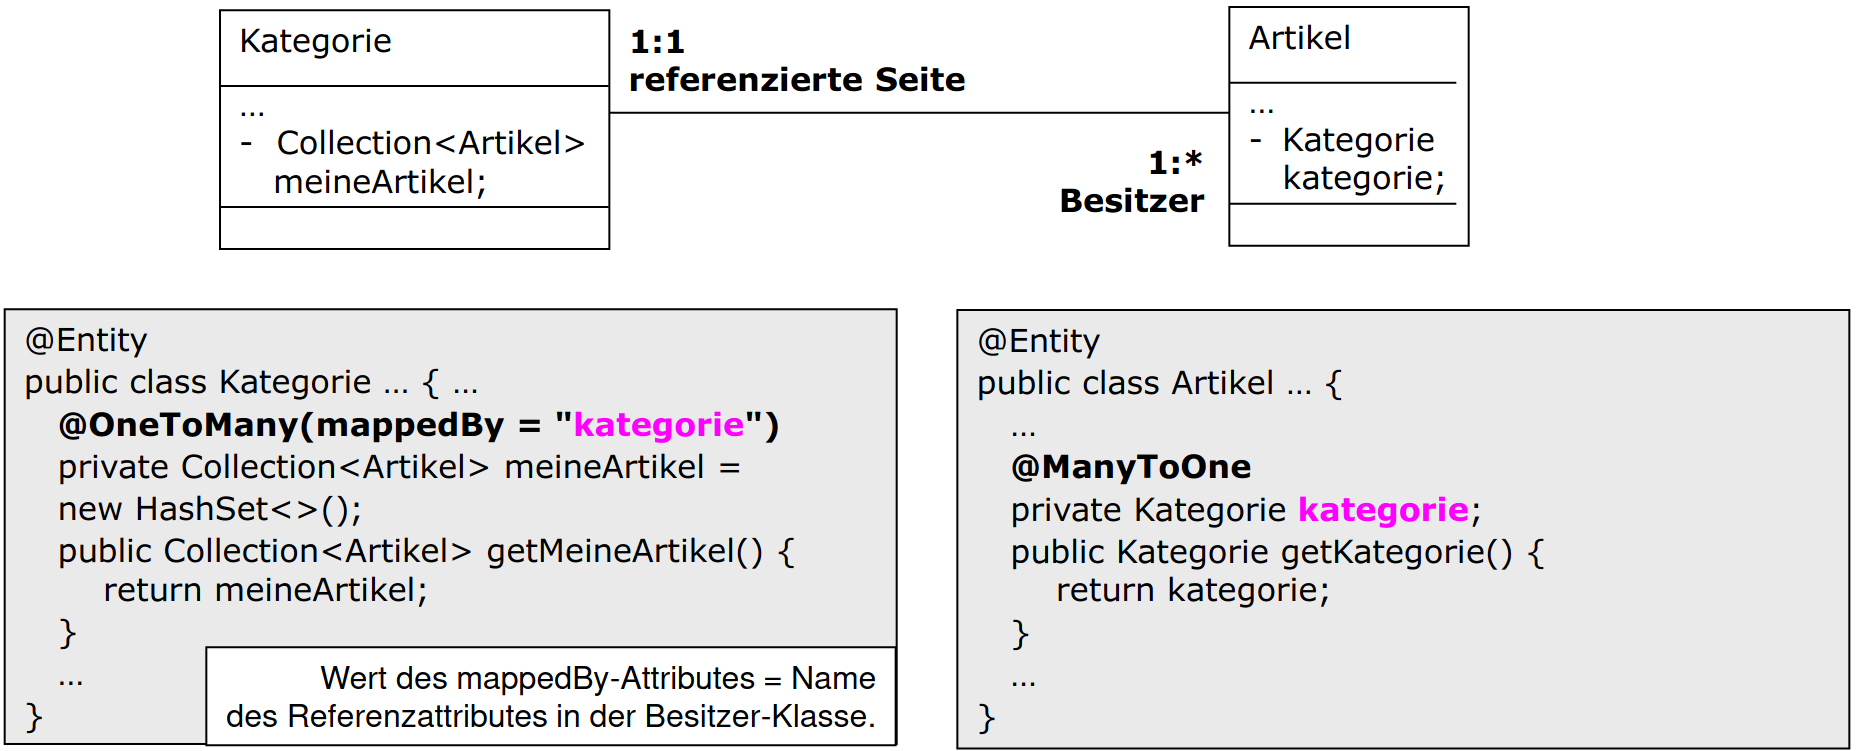
\includegraphics[width=500px]{JPAOneToMany.png}

1-n Beziehungen in Java direkt in 1-n Beziehungen in der DB zu mappen ist zwar laut der Spezifikation auch möglich, aber nicht empfehlenswert, da die Implementierung nicht korrekt ist. Im Beispiel würde dann bei unserem Klassendiagramm die Klasse Kategorie nur die \textit{@OneToMany} Annotation ohne den Zusatz von \textit{mappedBy} bekommen. Bei der Klasse Artikel würde dann die Referenz auf die Kategorie und damit auch die Annotation fehlen.\\
Das Problem hierbei ist, dass daraus dann in der DB tatsächlich keine 1:n Beziehung, sondern eine n:m Beziehung generiert werden würde. D.h. es würde eine Zwischentabelle erzeugt werden, die Kombinationen von Primärschlüsseln der beiden Tabellen als Fremdschlüssel speichert.


\subsubsection{n:m ManyToMany Beziehungen}
In Java können n:m Beziehungen, wie auch 1:n Beziehungen (siehe vorheriges Kapitel), sowohl unidirektional, als auch bidirektional dargestellt werden.\\
\textbf{Unidirektionale n:m Beziehung} würde bedeuten, dass wir genau wie bei einer unidirektionalen 1:n Beziehung eine umschließende Klasse haben, die eine Collection von Referenzen auf eine umschlossene Klasse enthält. Nur hier würden wir erlauben, dass wir eine Referenz auf ein und das selbe Objekt der umschlossenen Klasse in den Collections mehrerer verschiedener Objekte der umschließenden Klasse enthalten haben. Das heißt designtechnisch ist das Java Klassendiagramm genau wie für eine 1:n Beziehung, der Unterschied ist nur der Umgang damit.\\
\textbf{Bidirektionale n:m Beziehung} würde bedeuten, dass beide Klassen eine Collection allen mit Referenzen auf Objekte der anderen Klasse haben, denen sie zugeordnet sind.\\
\\

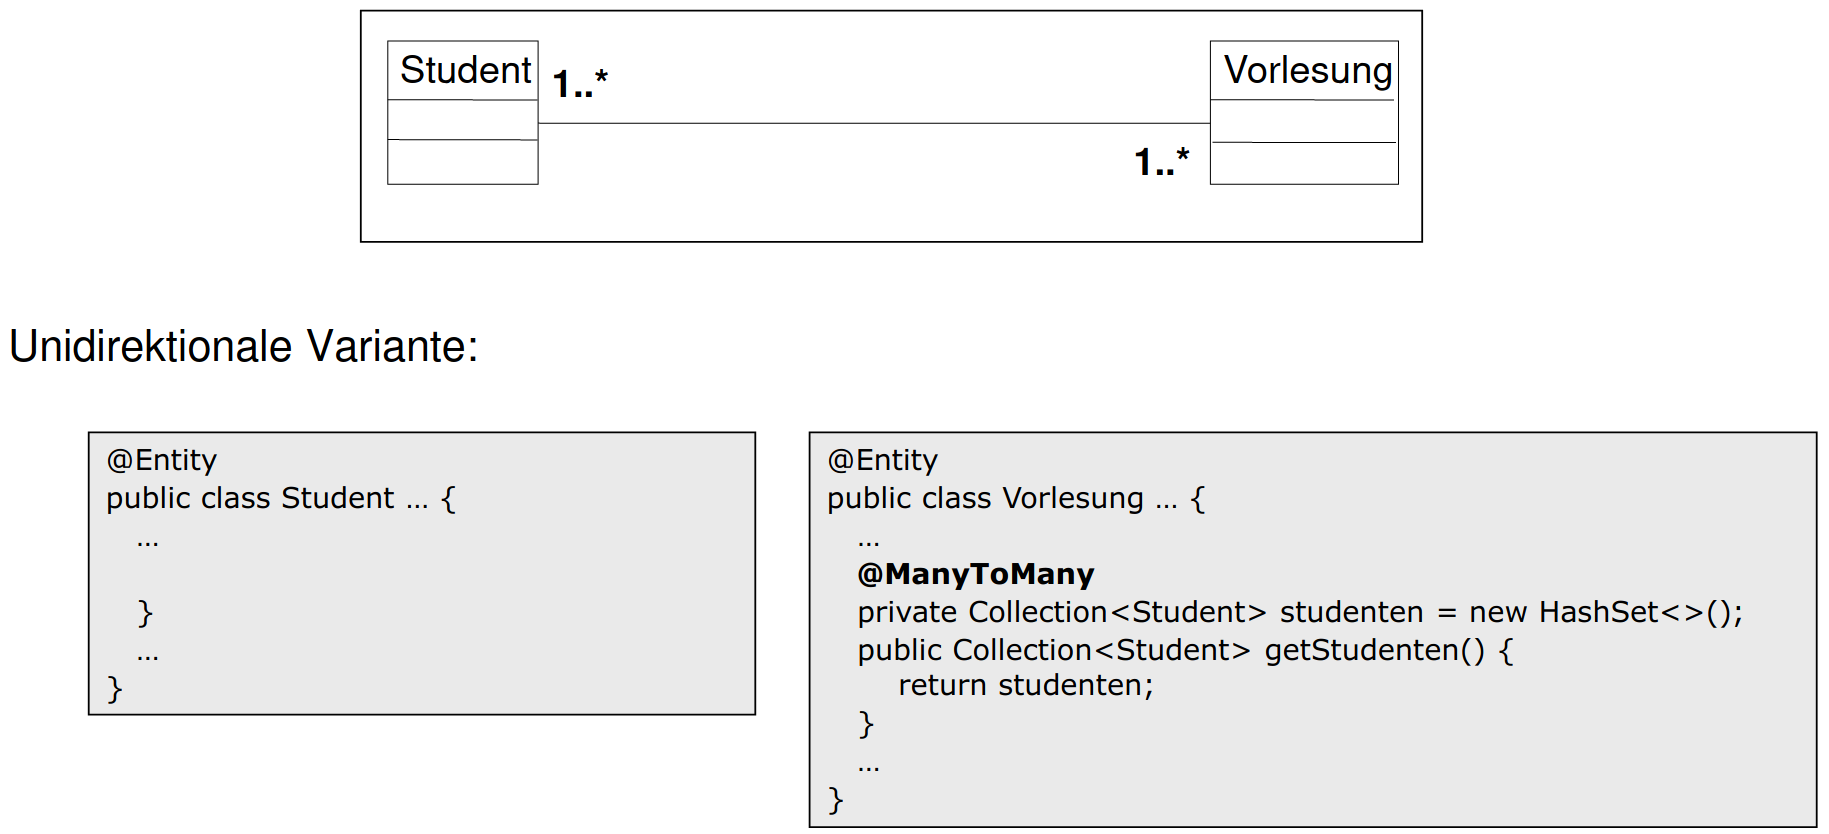
\includegraphics[width=400px]{JPAManyToManyUnidirectional.png}

Der unidirektionale Fall ist sehr einfach umgesetzt. Hier kann einfach die Annotation \textit{@ManyToMany} bei der Collection benutzt werden. Zusätzlich kann optional noch die Annotation \textit{@JoinTable(name=''table\_name'')} benutzt werden, um zu bestimmen, wie die Zwischentabelle in der DB, die die Beziehung abbildet, benannt werden soll. Es gibt auch noch andere Annotationen, mit denen auch die Namen der Attribute personalisiert werden können, auf die hier nicht weiter eingegangen wird.

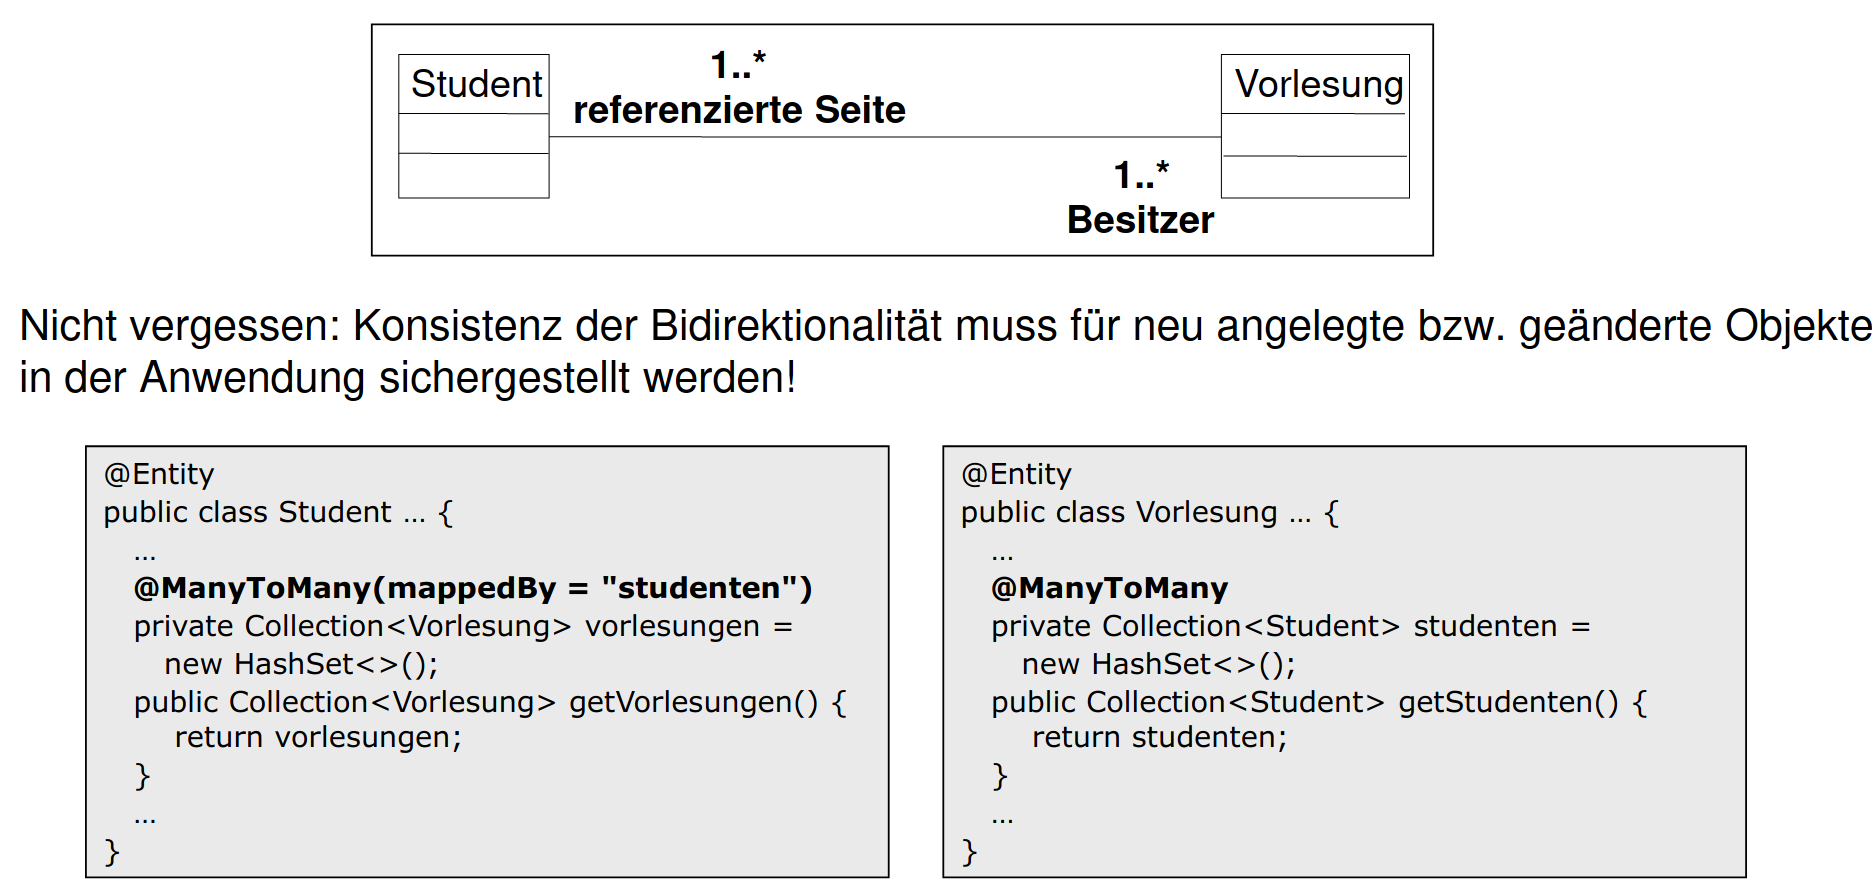
\includegraphics[width=400px]{JPAManyToManyBidirectional.png}

Bei der bidirektionalen Variante haben wir die Information über die Beziehung zwischen den Entity-Klassen doppelt gespeichert (und hoffentlich Konsistent). Deshalb müssen wir hier, wie auch bei der bidirektionalen 1:n Beziehung, auf einer Seite beim Referenzattribut mittels \textit{mappedBy = ''attribut\_name''} anzeigen, dass diese Beziehung bereits durch ein anderes Attribut mit dem Namen attribut\_name dargestellt wird. Das heißt JPA wird das so annotierte Attribut ignorieren. Dadurch entsteht für JPA eine unidirektionale Beziehung, die wie oben erklärt abgebildet wird. Für den Programmierer bleibt jedoch die Flexibilität der bidirektionalen Beziehung bestehen.


\subsubsection{Kompositionen komplexer Typen und Collections}
Zuvor haben wir nur primitive Datentypen als Komposition darstellen können. Für andere Datentypen wurde mit den Annotationen \textit{@OneToMany} eine Assoziation erstellt. Um auch Kompositionen von Komplexen Typen darstellen zu können müssen wir den Typ, der eingebettet sein soll, statt mit \textit{@Entity} mit \textit{@Embeddable} annotieren. Wird dieser Typ dann in einer umschließenden Klasse als Komposition benutzt, so muss dieses Attribut als \textit{@Embedded} annotiert werden.\\
Der Unterschied zu einer Assoziation einer mit \textit{@Entity} annotierten Klasse ist dabei, dass das Hinzufügen und Löschen von Objekten der umschließenden Klasse zur umschlossenen Klasse kaskadieren, so wie wir es in OO-Programmiersprachen von Kompositionen gewöhnt sind.\\

Im Fall von einem einzigen \textit{@Embedded}-Attribut werden alle Attribute der eingebetteten Klasse in der Datenbank als Attribute der umschließenden Klasse angelegt. Im Falle einer \textit{@EmbeddedCollection} wird eine separate Relation benötigt.

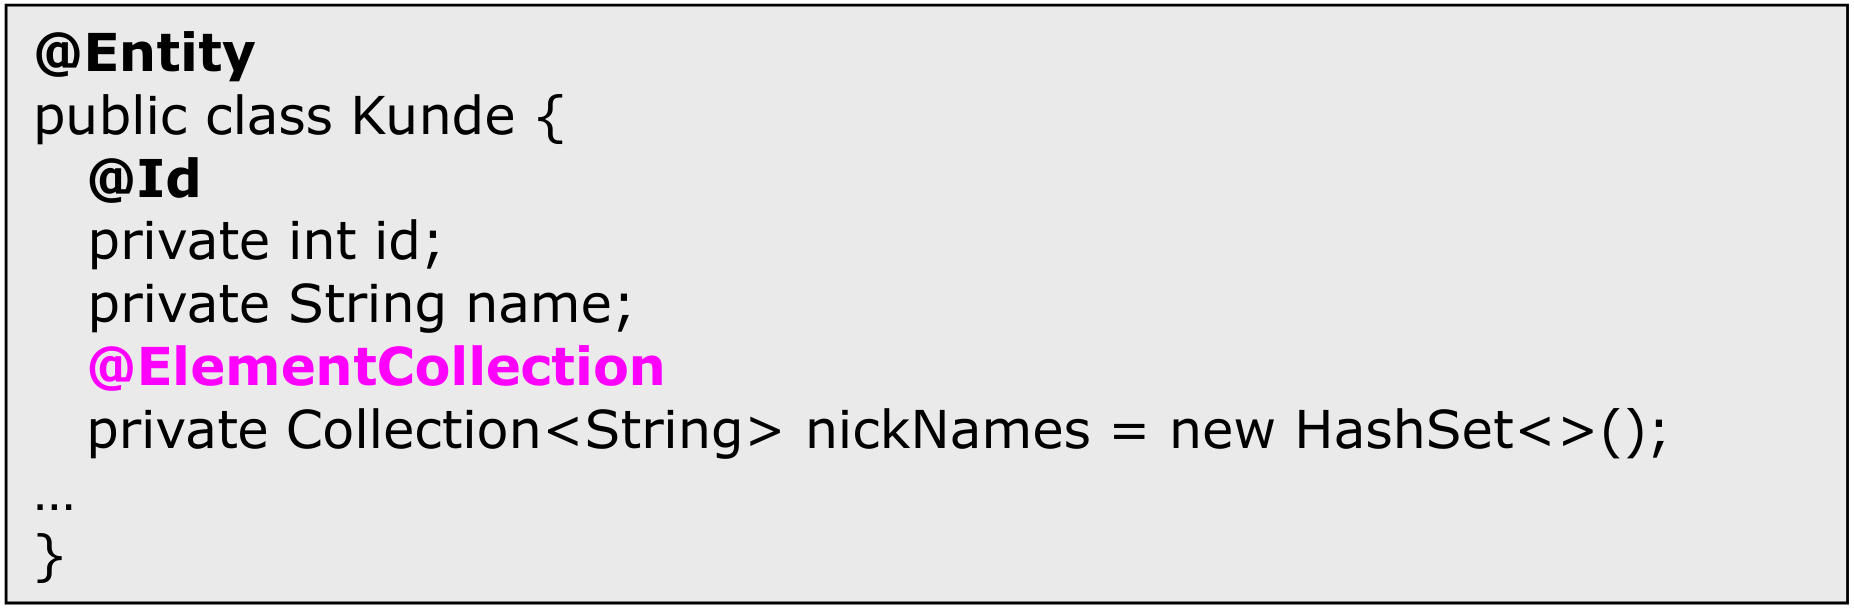
\includegraphics[width=300px]{JPAElementCollection.png}

\textbf{Collections} können als \textit{@EmbeddedCollection} annotiert werden, um eine Komposition einer Collection herbeizuführen. Dabei muss der Typ der Collection ein primitiver Typ, den in in der DB auch gibt, oder eine mit \textit{@Embeddable} annotierte Klasse sein. Tatsächlich wird in der DB sehr wohl eine weitere Tabelle angelegt, um das zu bewerkstelligen, aber diese wird so abstrahiert, dass die Collection in der Java-Anwendung als Komposition betrachtet werden kann. Dabei ist zu beachten, dass mit \textit{@Embeddable} annotierte Klassen keine \textit{@Id}-Annotation benötigen.

\subsubsection{Inheritance}
die in OO-Programmiersprachen und im Relationenmodell bekannte Inheritance (Vererbung) gibt es so in relationalen Datenbanken nicht. Doch man kann Vererbung auf 3 verschiedene Weisen abbilden lassen. Um JPA mitzuteilen, welche Strategie angewendet werden soll, wird in der Elternklasse die Annotation \textit{\textbf{@Inheritance(strategy = InheritanceType.XXXX)}} benutzt. Die verschiedenen Strategien werden hier kurz erläutert:
\begin{itemize}
    \item \textbf{InheritanceType.JOINED}: Für jede Klasse, auch für Superklassen, wird eine Tabelle erstellt. Wenn alle Instanzen der einer abstrakten Klasse benötigt werden, also z.B. alle Bücher (Audiobooks, Taschenbücher...) muss nur die Tabelle für die abstrakte Klasse durchsucht werden. Allerdings werden selbst für den Zugriff auf Daten einer abgeleiteten Klasse JOINS benötigt, weil einige Attribute aus dem Table, der der Superklasse zugeordnet ist, geholt werden müssen.
    \item \textbf{InheritanceType.SINGLE\_TABLE}: Für alle Klassen der Vererbunghierarchie wird nur ein gemeinsamer Table angelegt. Zeilen haben dann NULL Werte an den Attributen, die es in der Klasse, der sie entstammen, nicht gab. Der Vorteil ist der schnelle Zugriff ohne JOINS. Der Nachteil ist die Verschwendung von Speicherplatz für die NULL Werte.
    \item \textbf{InheritanceType.TABLE\_PER\_CLASS}: Erstellt für jede konkrete Klasse eine Tabelle. Attribute von abstrakten Superklassen werden in den Tabellen der abgeleiteten Klassen eingefügt. Wenn man alle Datensätze, die zu Subtypen einer abstrakten Klasse gehören, muss man nun mehrere Tabellen, nämlich so viele, wie es abgeleitete Klassen gibt, durchsuchen. Diese Strategie ist in JPA optional spezifiziert und wird nicht von allen Frameworks implementiert.

\end{itemize}

\subsection{Funktionsweise des Frameworks}
\subsubsection{Entity-Lifecycle}
\vspace{5px}
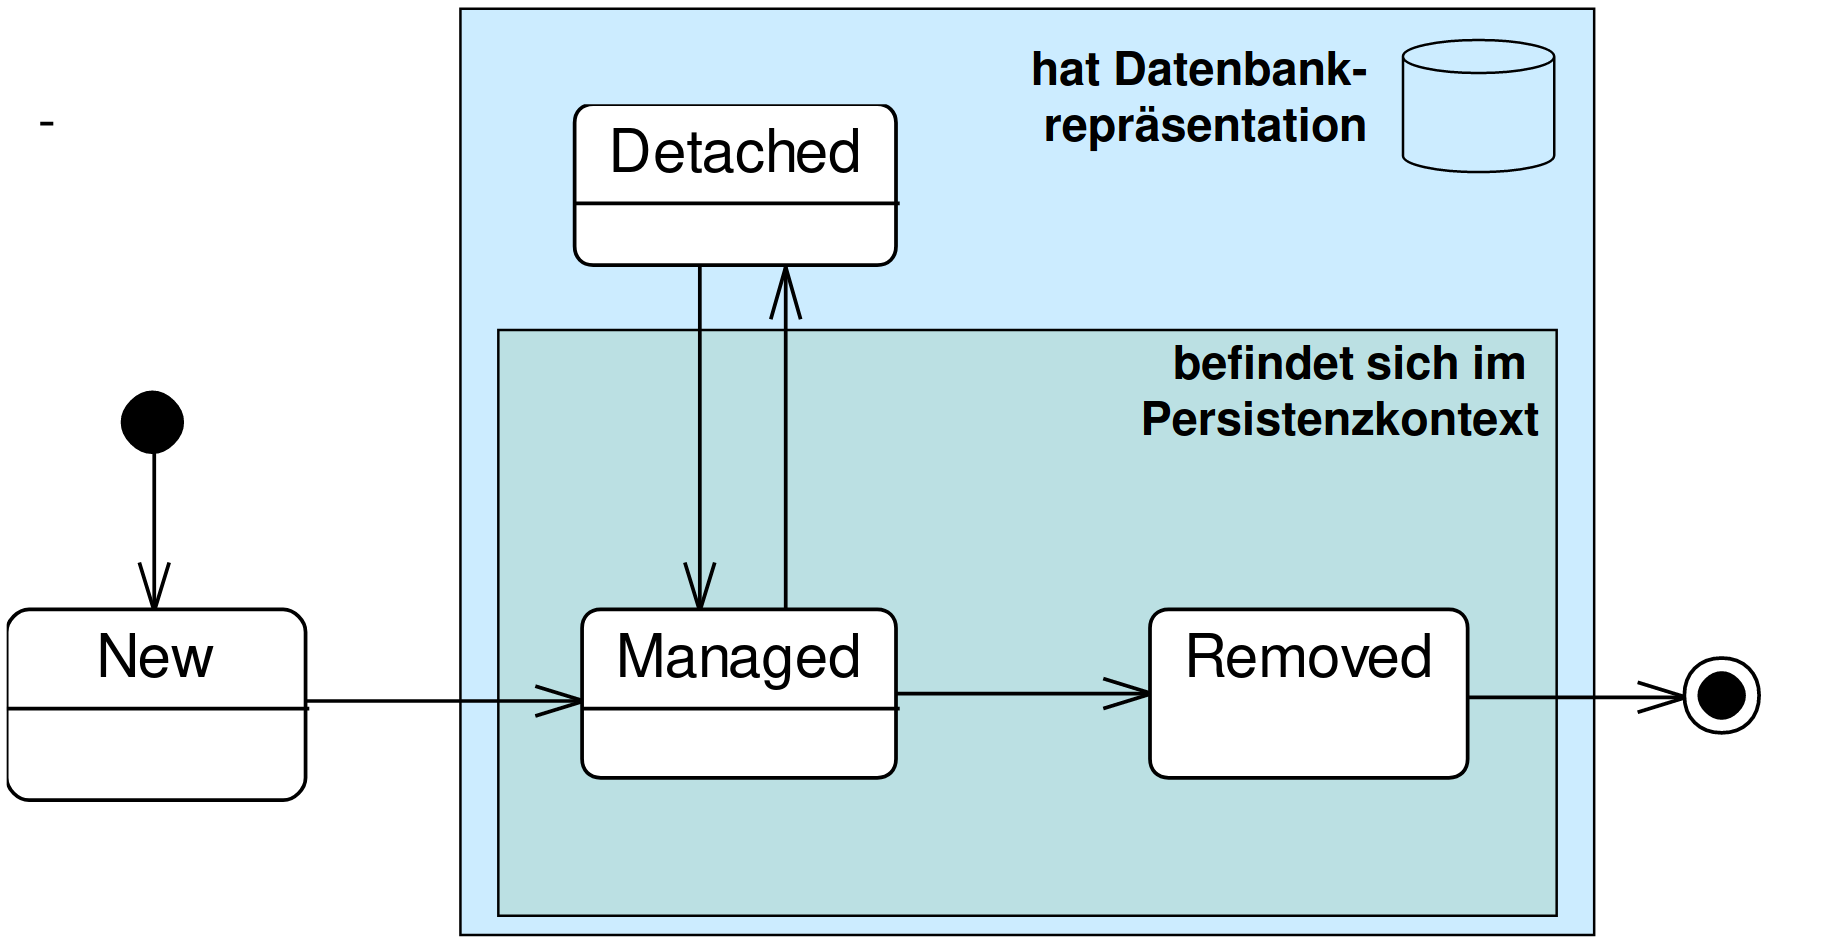
\includegraphics[width=400px]{JPAEntityLifecycle.png}

Eine Instanz einer Entity-Klasse kann sich in 4 verschiedenen Zuständen befinden:
\begin{itemize}
    \item \textbf{New}: Wenn ein Objekt erzeugt wird, ist es zunächst nicht im Persistenzkontext. Es ist in dieser Zeit also nur ein einfaches, vom OR-Framework unabhängiges Objekt.
    \item \textbf{Managed}: Das Objekt befindet sich im Persistenzkontext. Es hat 0-1 relationale Repräsentation in der DB (keine falls es gerade erst dem Persistenzkontext hinzugefügt wurde und die Änderung noch nicht commitet wurde). Änderungen an dem Objekt werden beim nächsten Commit mit der Datenbank synchronisiert.
    \item \textbf{Detached}: Das Objekt hat eine Repräsentation in der Datenbank, befindet sich aber nicht im Persistenzkontext, wird also zurzeit nicht mehr vom EntityManager verwaltet. Es ist also wieder unabhängig vom ER-Framework.
    \item \textbf{Removed}: Das Objekt soll aus der Datenbank gelöscht werden. Beim nächsten Commit wird die Repräsentation dann aus der Datenbank gelöscht und es wird aus dem Persistenzkontext genommen.
\end{itemize}

Um Objekte zwischen den verschiedenen Zuständen zu bewegen, gibt es Methoden der EntityManager-Class. Einige sollen im Folgenden vorgestellt werden:
\begin{itemize}
    \item \lstinline{void persist(Object obj)}: Nimmt ein Objekt in den Persistenzkontext auf.
    \item \lstinline{T find(Class<T> entityClass, Object primaryKey)}: Sucht eine Entity anhand ihres Primary Keys im Persistenzkontext. Falls es nicht gefunden wird, sucht es das Objekt in der Datenbank. Falls gefunden, wird das entsprechende Objekt zurückgegeben, andernfalls \textbf{null}.
    \item \lstinline{T getReference(Class<T> entityClass, Object obj)}: wie find(), nur das eventuell bloß eine noch im Cache vorhandene Version geladen wird, die eventuell dirty ist.
    \item \lstinline{boolean contains(Object obj)}: Gibt zurück, ob ein Objekt im Persistenzkontext ist
    \item \lstinline{void refresh(Object obj)}: Aktualisiert das Objekt im Persistenzkontext durch Nachladen seiner relationalen Repräsentation in der DB. D.h. falls die Daten in der DB inzwischen durch andere parallelle Prozesse geändert wurden, kann der Persistenzkontext aktualisiert werden.
    \item \lstinline{void remove(Object obj}: Schiebt eine Entity in den Zustand removed (siehe oben).
    \item \lstinline{void flush()}: Erzwingt die Abwärtssynchronisation von Hauptspeicher nach DB schon vor dem Commit.
    \item \lstinline{void detach(T entity)}: Schiebt ein Objekt in den Zustand detached, es befindet sich dann nicht mehr im Persistenzkontext.
    \item \lstinline{T merge(T entity)}: Fügt eine Copy eines detached Objektes wieder in den Persistenzkontext ein und gibt eine Referenz auf das eingefügte Objekts zurück.
    \item \lstinline{ void clear()}: Detached alle Objekte.
\end{itemize}

\subsubsection{Transaktionen und Sessions}
\begin{itemize}
    \item Beim Erzeugen eines EntityManagers über EntityManagerFactory.getEntityManager() wird eine DB-Session für diesen EntityManager eröffnet.
    \item Beim Aufruf von EntityManager.close() wird die DB-Session dieses EntityManagers geschlossen.
    \item Beim Aufruf von EntityManager.getTransaction().begin() wird eine Transaktion innerhalb der Session des EntityManagers gestartet.
    \item Beim Aufruf von EntityManager.getTransaction().commit() wird diese Transaktion beendet.
\end{itemize}

\subsubsection{Transitive Persistenz}
Normalerweise beziehen sich die Funktionen persist(), merge(), remove() ,refresh() und detach() nur auf das Objekt, mit dem sie aufgerufen werden. Also nicht für Objekte, die als Attribute mit @ManyToOne, @OneToMany, @ManyToMany, @OneToOne enthalten sind. Für diese müssen die Funktionen gesondert aufgerufen werden. Um die Funktionsaufrufe zu kaskadieren und damit auch für die referenzierten Objekte auszuführen, kann man noch den Zusatz cascade = CascadeType.XXXX hinzufügen.\\
Bsp.:\\
\textbf{@OneToMany( cascade = CascadeType.PERSIST)}

\subsubsection{Callback Methoden}
Methoden einer Entity-Class können mit bestimmten Annotationen als Callback Methoden für Aufrufe von bestimmte Methodenaufrufe der EntityManager Klasse eingetragen werden. Der Effekt ist ähnlich dem von Triggern:
\begin{itemize}
    \item @PrePersist
    \item @PostPersist
    \item @PostLoad
    \item @PreUpdate
    \item @PostUpdate
    \item @PreRemove
    \item @PostRemove
\end{itemize}